\begin{tikzpicture}
\def \Lq{0.5\linewidth}
\def \offset{-0.01\linewidth}
\node at (0, 0) {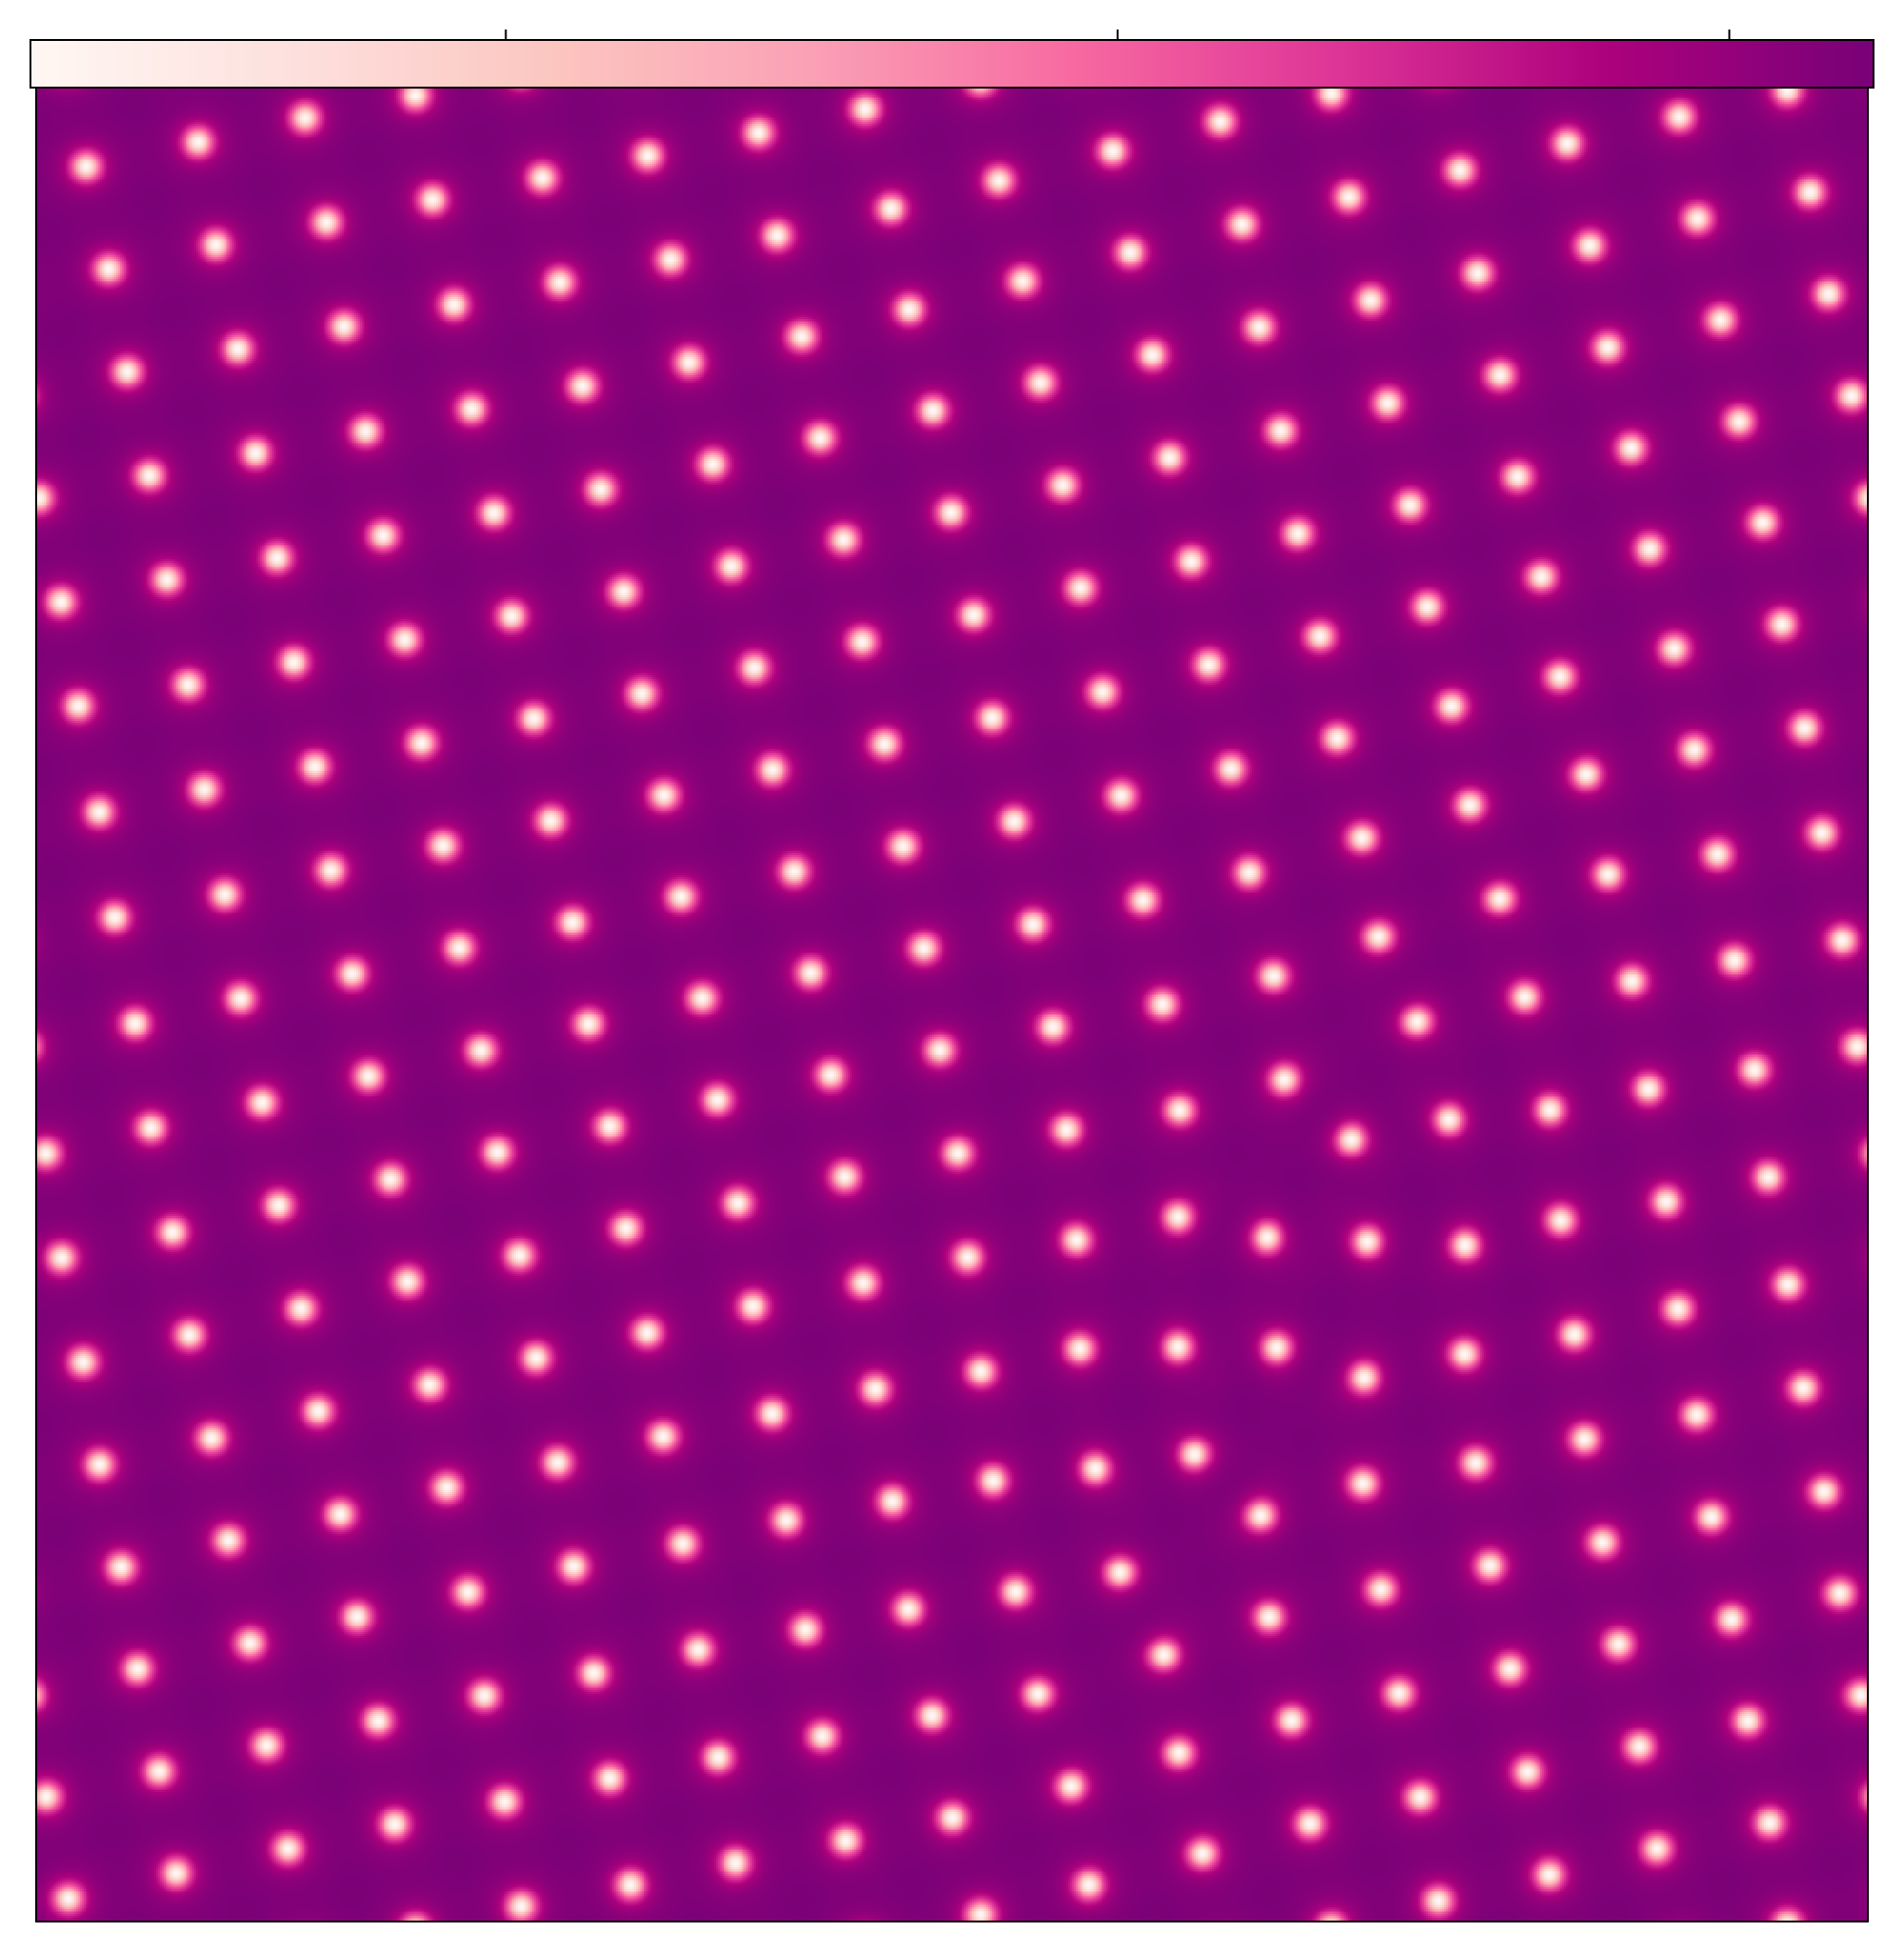
\includegraphics[width=0.48\linewidth]{density.png}};
\node at (0, 0.505*\Lq) {Density $\rho$};
\node at (-0.4*\Lq, 0.505*\Lq) {$0.67$};
\node at (0.42*\Lq, 0.505*\Lq) {$0.7$};
\node[text = black, rectangle, rounded corners=3pt, fill=white, opacity=0.75] at (-0.38*\Lq, 0.38*\Lq) {(a)};

\node at (\Lq, 0) {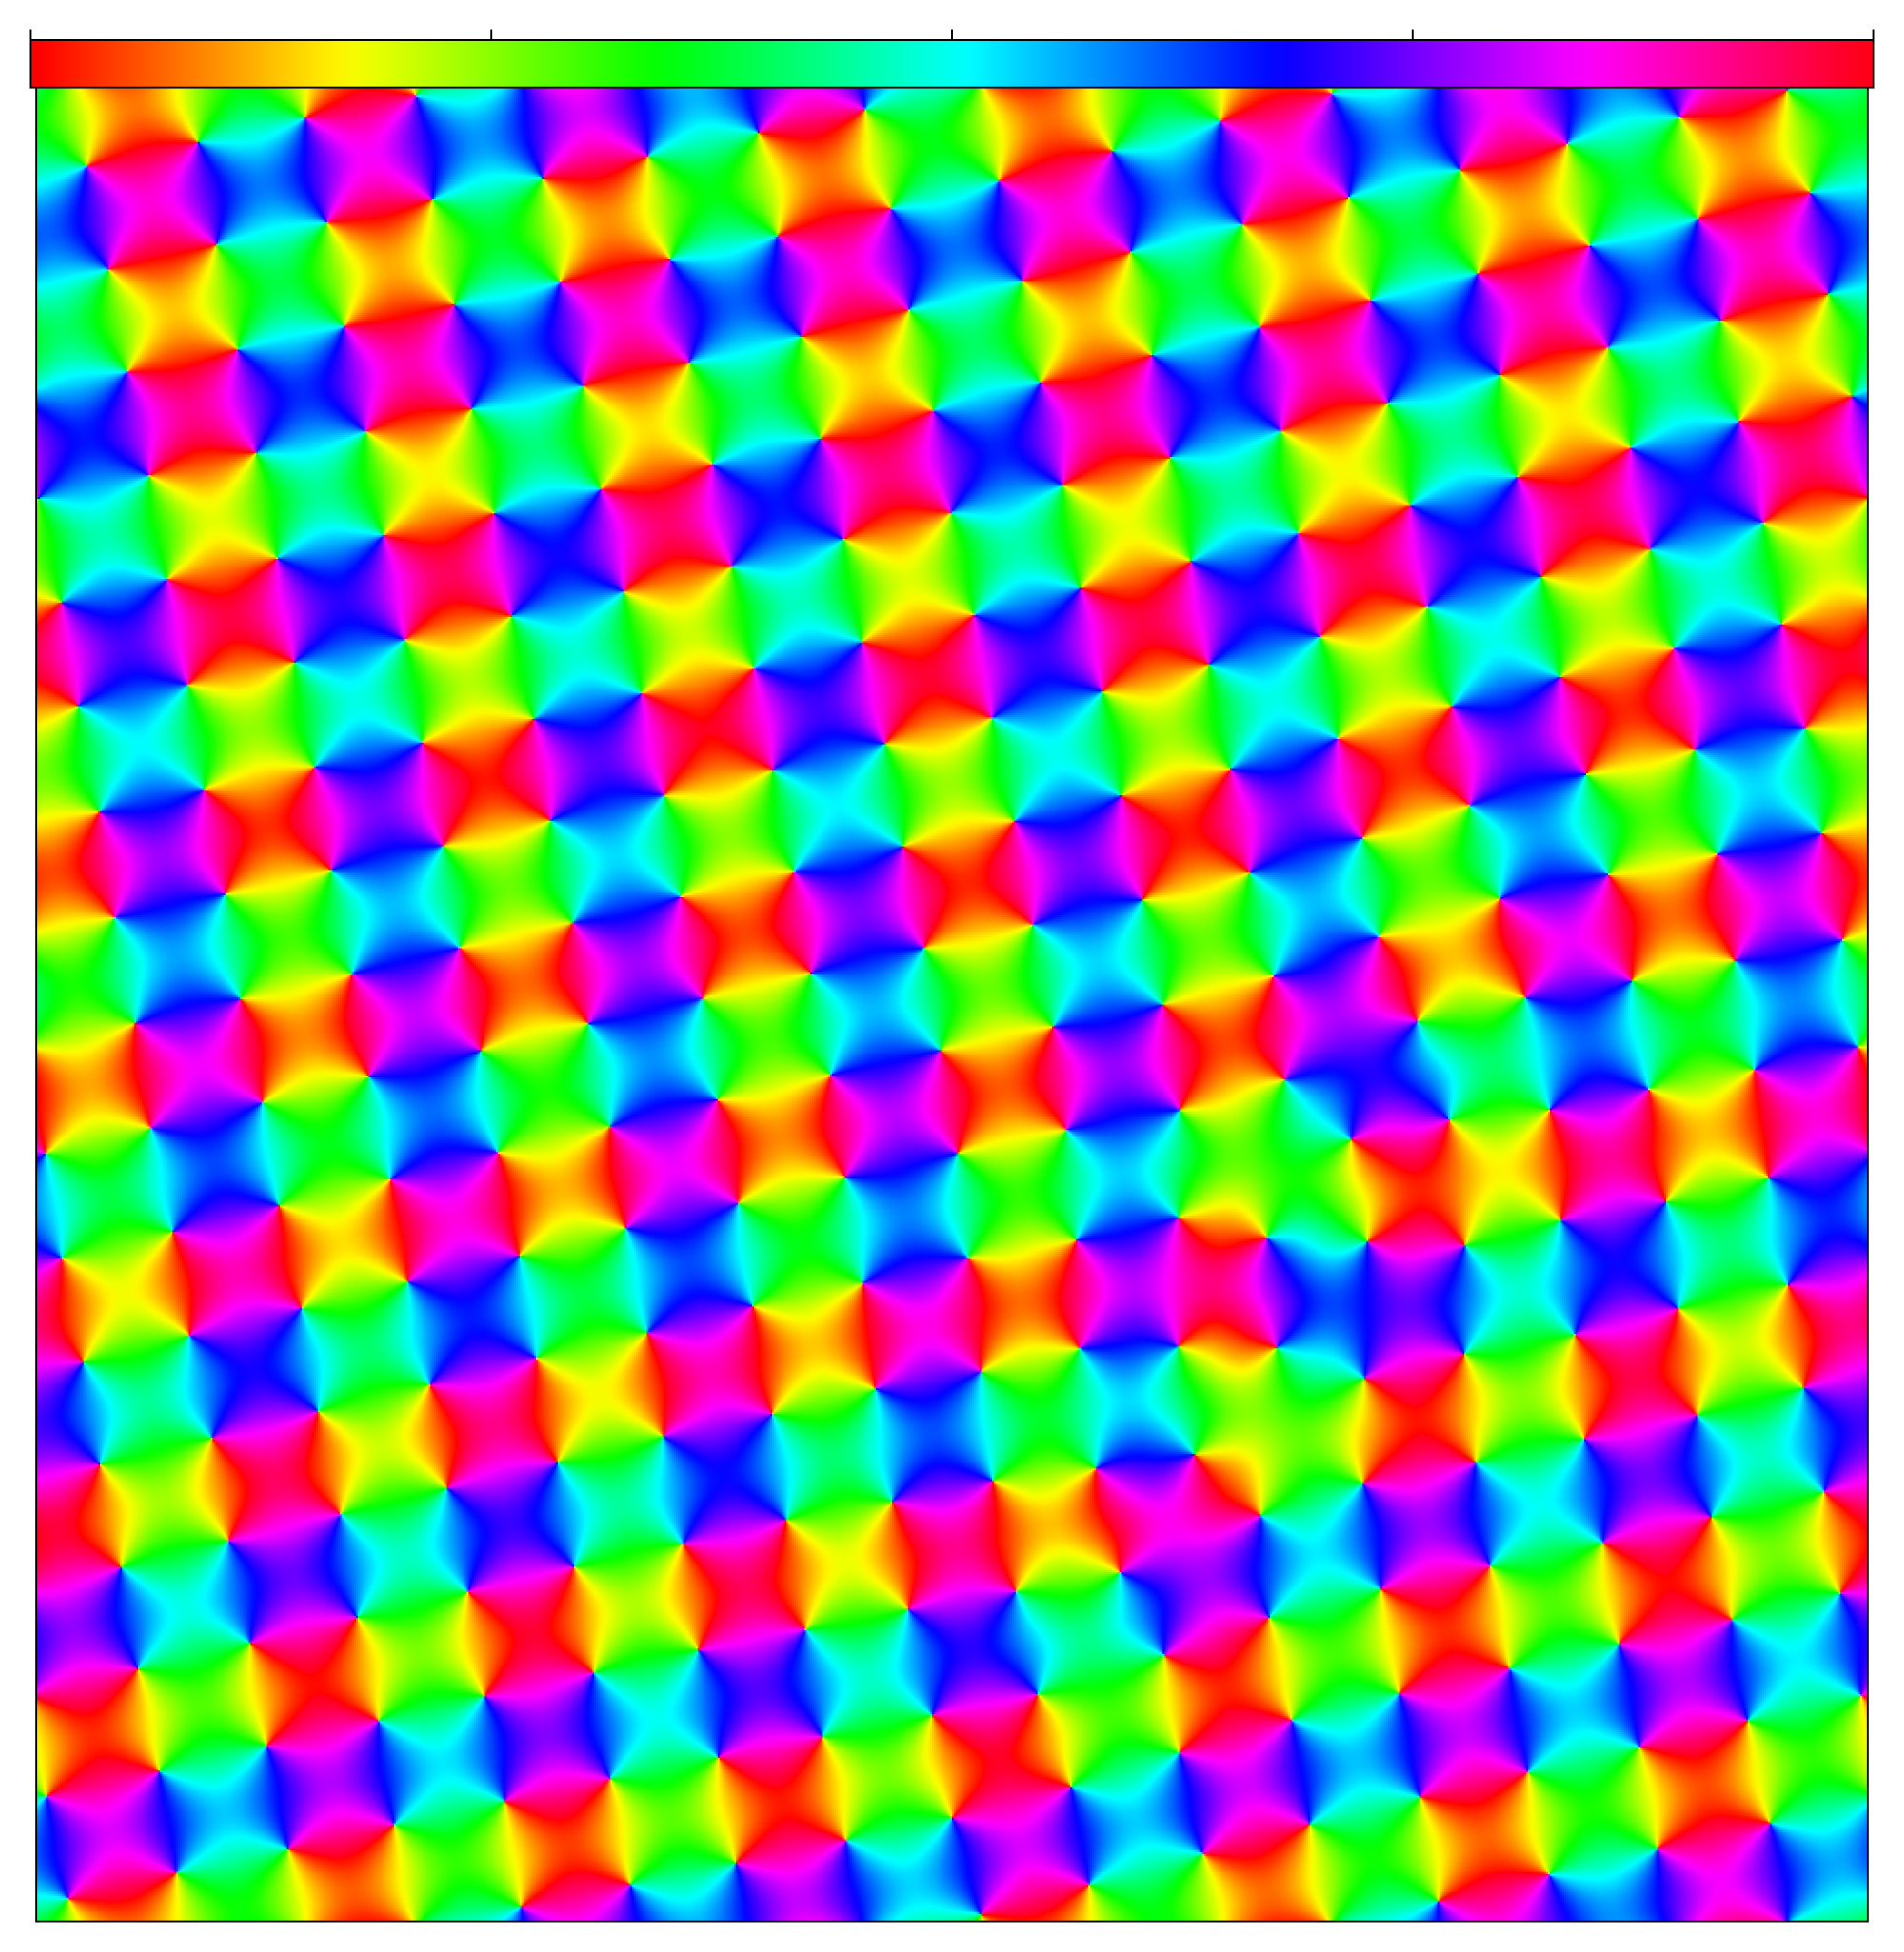
\includegraphics[width=0.48\linewidth]{angle.png}};
\node at (\Lq-0.45*\Lq, 0.505*\Lq) {$-\pi$};
\node at (\Lq, 0.505*\Lq) {Angle $\theta$};
\node at (\Lq+0.45*\Lq, 0.505*\Lq) {$\pi$};
\node[text = black, rectangle, rounded corners=3pt, fill=white, opacity=0.75] at (\Lq-0.38*\Lq, 0.38*\Lq) {(b)};

\node at (0, -1.0*\Lq+\offset) {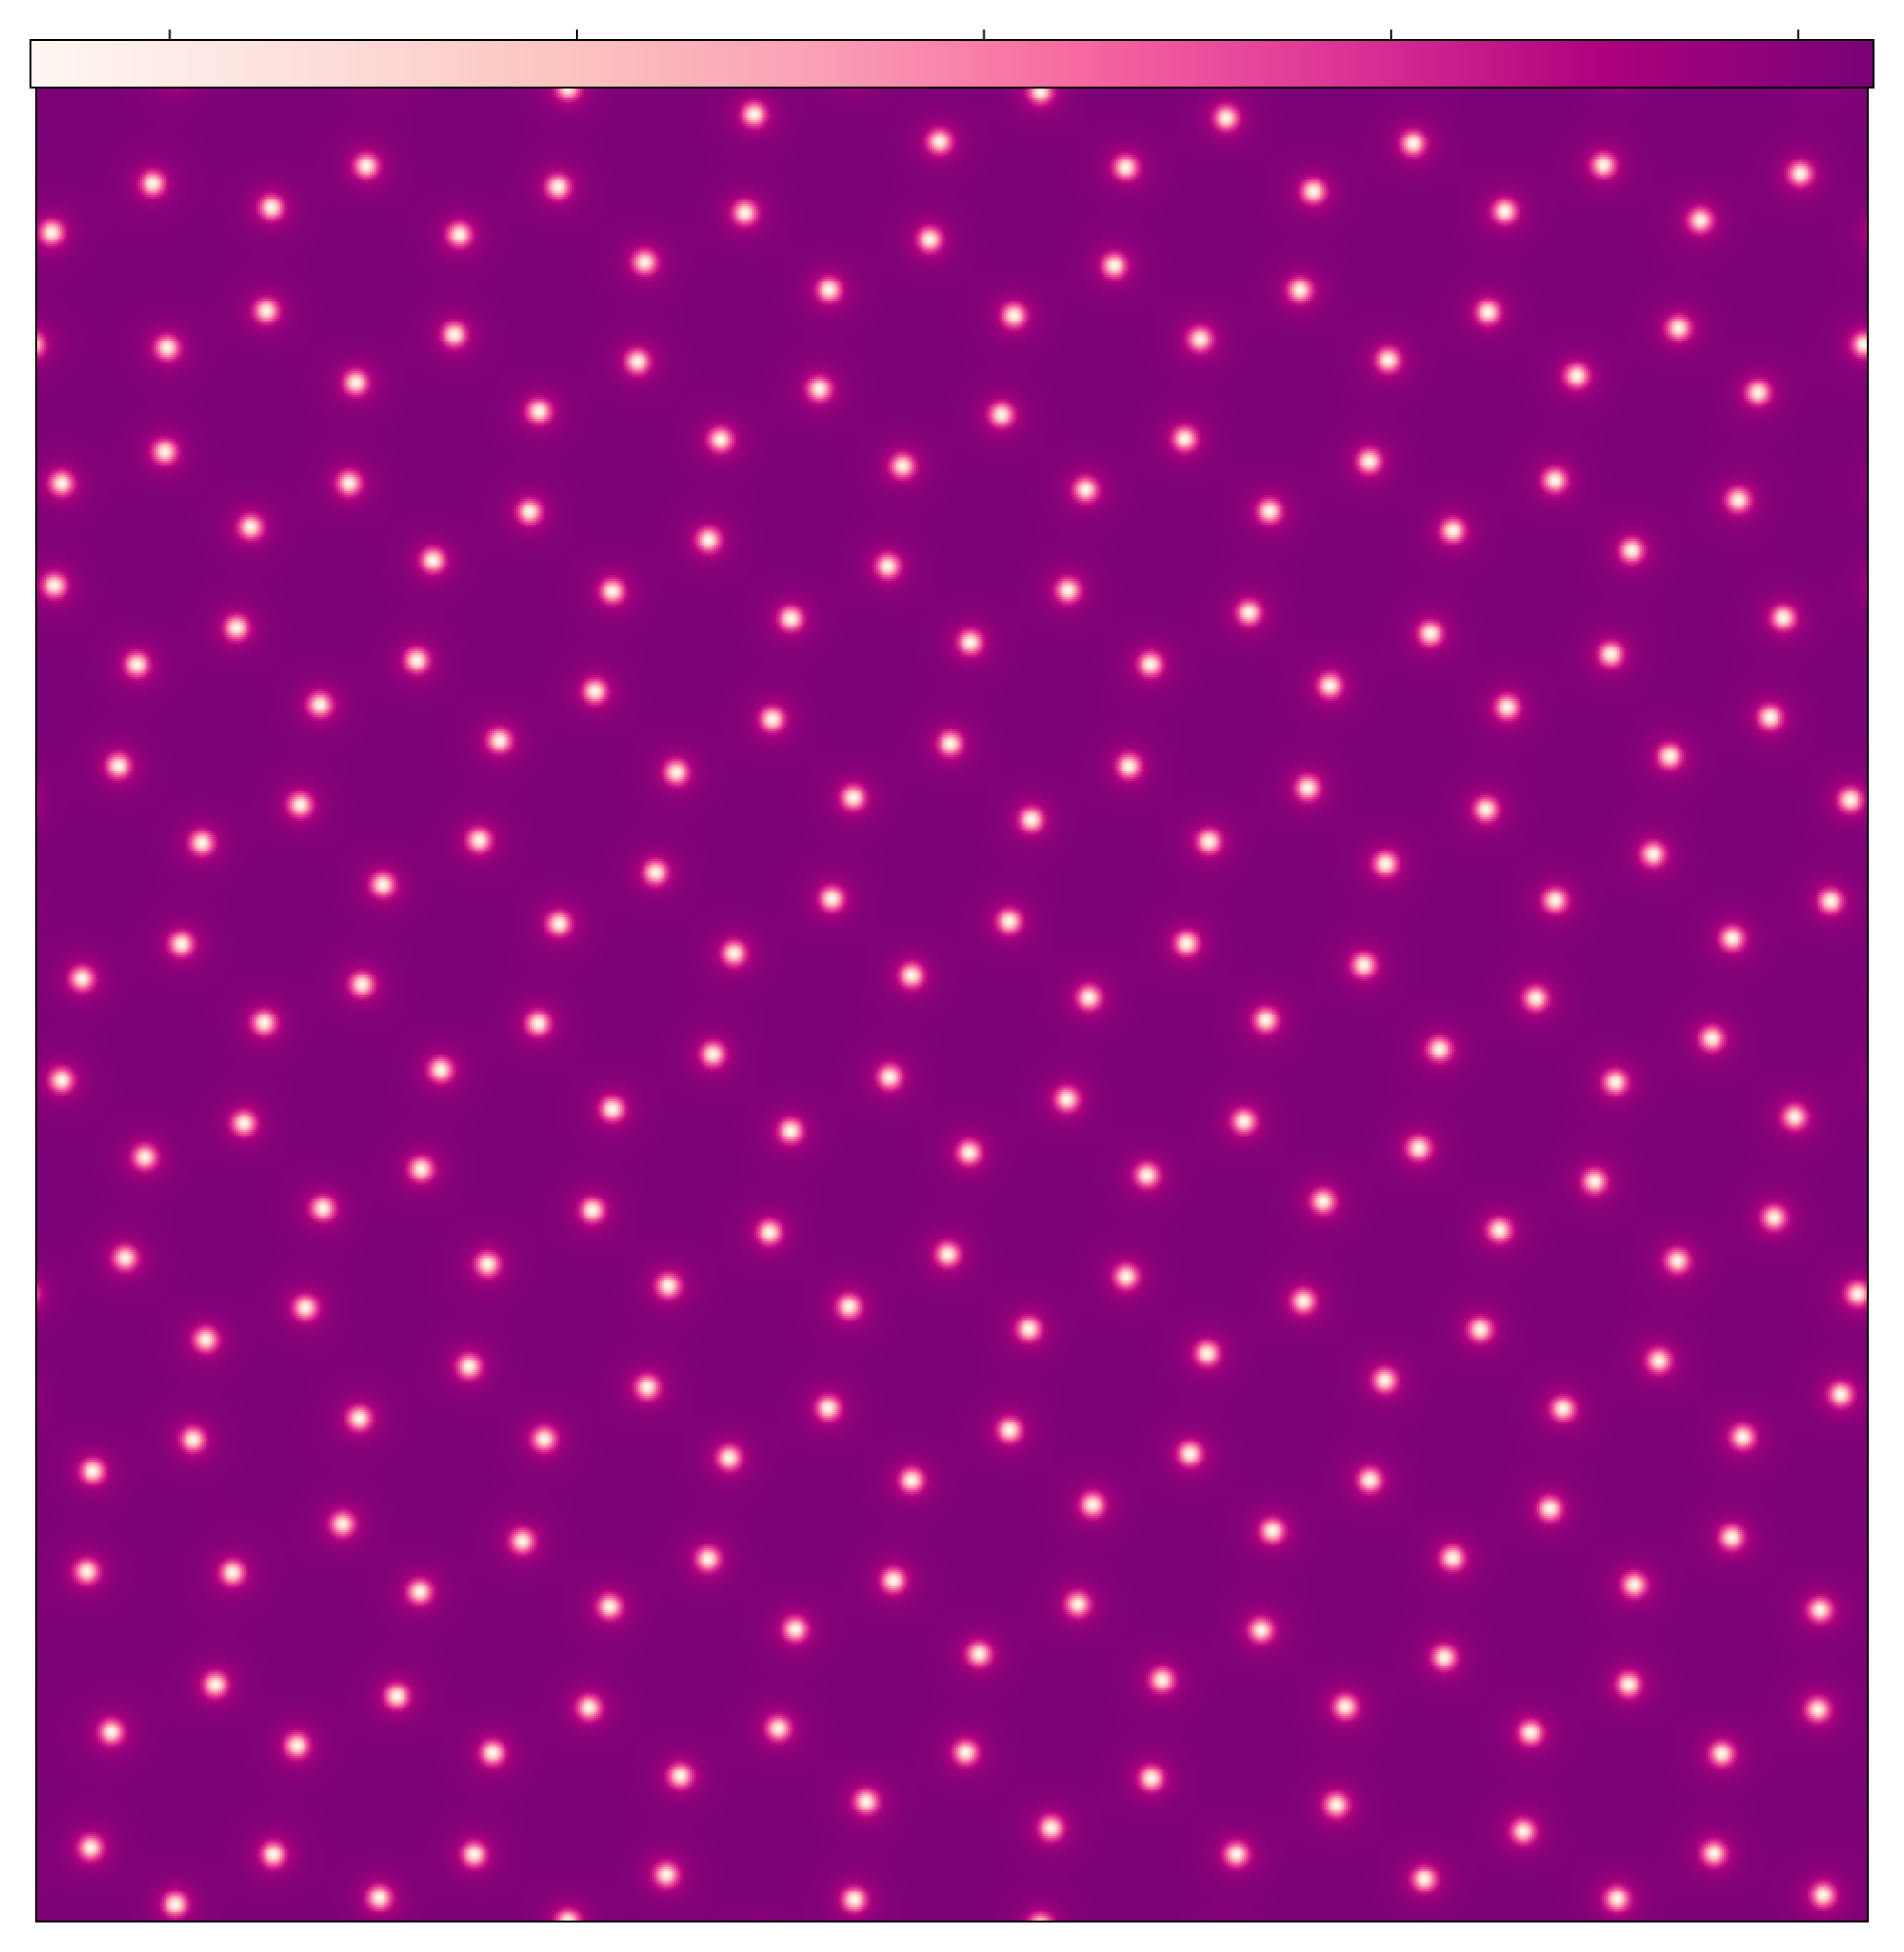
\includegraphics[width=0.48\linewidth]{density-2.png}};
\node at (0, 0.505*\Lq-\Lq+\offset) {Density $\rho$};
\node at (-0.42*\Lq, 0.505*\Lq-\Lq+\offset) {$1.28$};
\node at (0.42*\Lq, 0.505*\Lq-\Lq+\offset) {$1.3$};
\node[text = black, rectangle, rounded corners=3pt, fill=white, opacity=0.75] at (-0.38*\Lq, 0.38*\Lq-\Lq+\offset) {(c)};

\node at (\Lq, -1.0*\Lq+\offset) {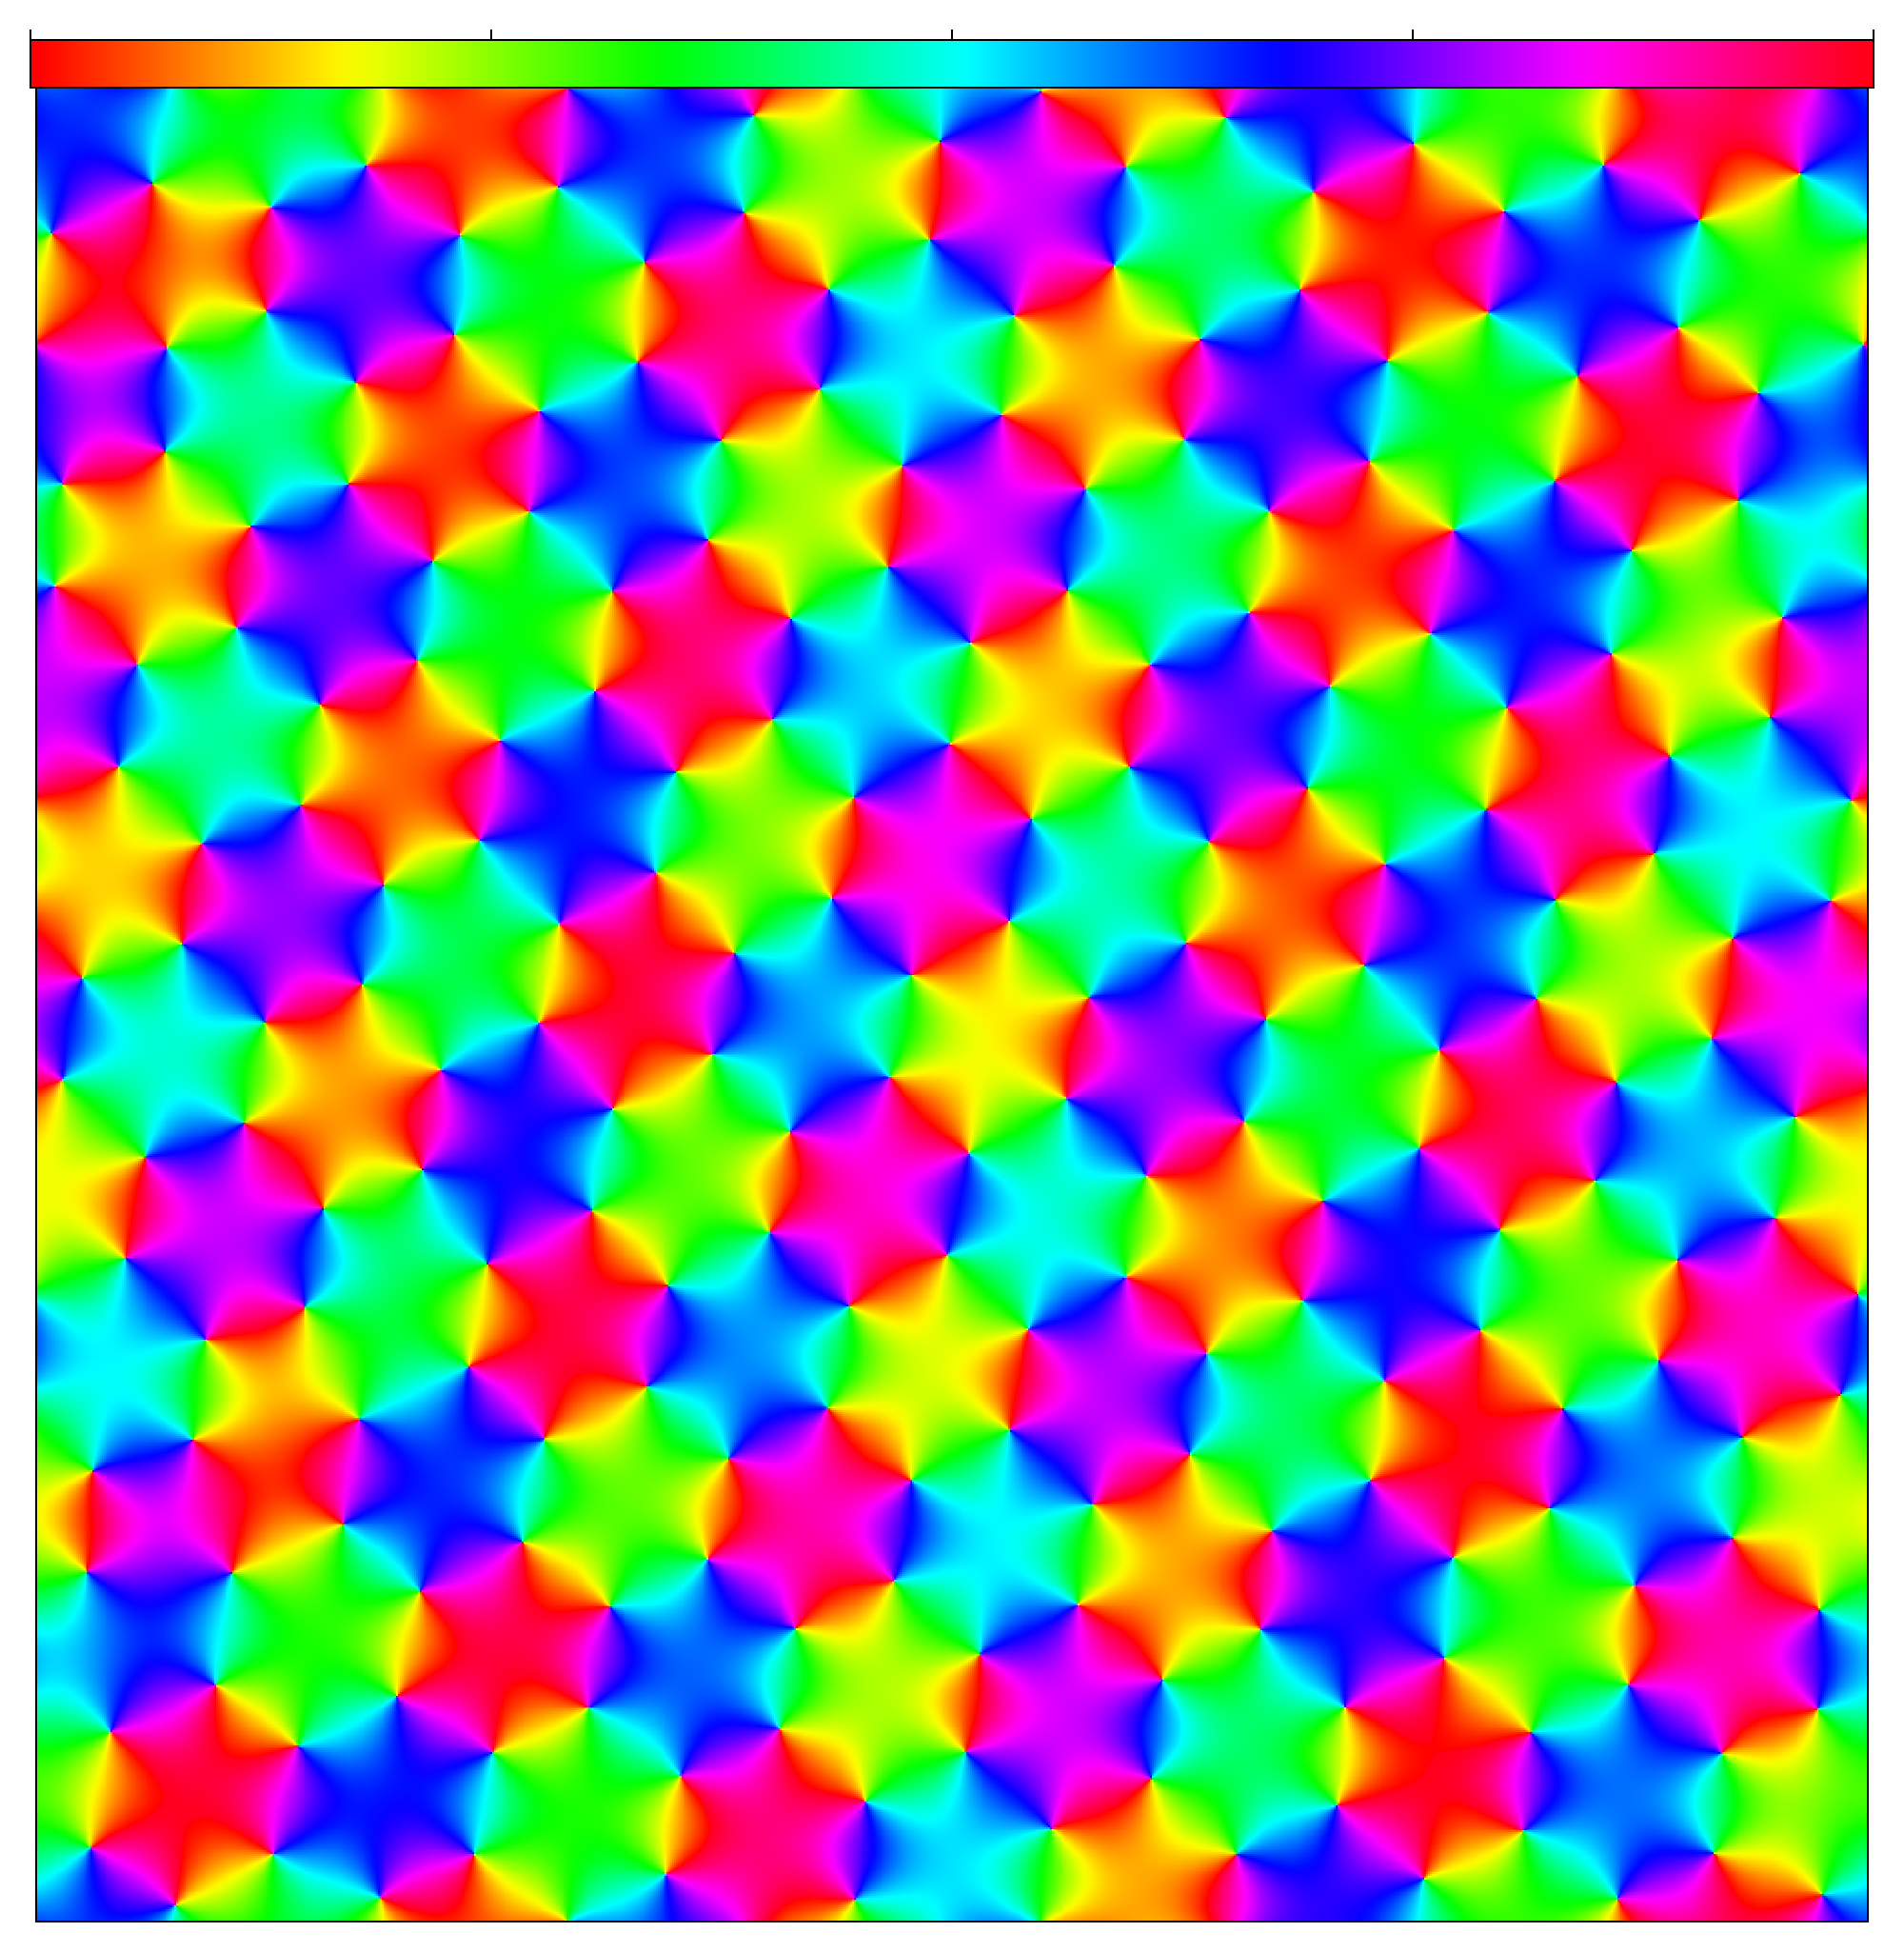
\includegraphics[width=0.48\linewidth]{angle-2.png}};
\node at (\Lq-0.45*\Lq, 0.505*\Lq-\Lq+\offset) {$-\pi$};
\node at (\Lq, 0.505*\Lq-\Lq+\offset) {Angle $\theta$};
\node at (\Lq+0.45*\Lq, 0.505*\Lq-\Lq+\offset) {$\pi$};
\node[text = black, rectangle, rounded corners=3pt, fill=white, opacity=0.75] at (\Lq-0.38*\Lq, 0.38*\Lq-\Lq+\offset) {(d)};
\end{tikzpicture}



% \begin{figure}
% \bc
% \includegraphics[width=\linewidth]{Fig/Fig_SquareLattice.pdf}
% \includegraphics[width=\linewidth]{Fig/Fig_TriLattice.pdf}
% \ec
% \caption{Defect lattices. (a,b) Density for $\rho_0 = 0.7$, $\tau = 1$, and $\zeta_\rho=10$ (a) and $\rho_0 = 1.3$, $\tau = 0.2$, and $\zeta_\rho=1$ (b). (c,d) Angle of the polar field corresponding to (a) and (b). System of length $L=10$, other parameters as in Table~\ref{tab:parameterValues}. The evolution of the shape order is given in Fig.~\ref{fig:lattice1extended}} \label{fig:lattice1}
% \end{figure}